%\documentclass[a4paper,11pt]{report}


%\usepackage{graphicx}
%\usepackage{color} 
%\usepackage[dvipsnames]{xcolor}
%\colorlet{purple}{purple}

%\begin{document}


\section{\color{olive}Exercise 4: Behaviour Analysis of Circuits Including a 74HC02 Gate}

The 74HC02 is an integrated circuit of NOR gates. Firstly, the propagation delays and the transition times are measured for this gate in a no-load output condition. Then these parameters are measured in the case in which the gate is connected in the circuit in Figure \ref{comps}.

\begin{figure}[h!]
\centering
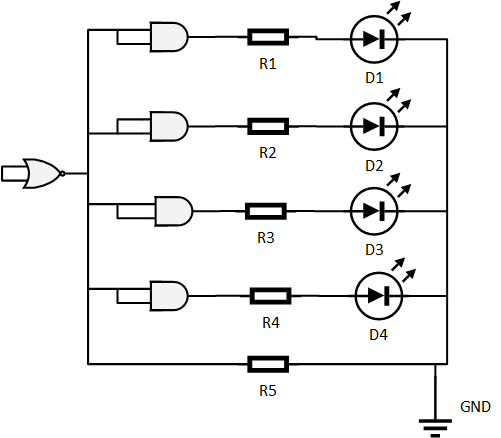
\includegraphics[scale=0.7]{../Exercise4/E3tp2ej4}
\caption{\color{cyan}74HC02 connected to a circuit with ANDS and leds.}
\label{comps}
\end{figure}

\subsubsection{\color{red}Propagation and Transition Times' Measurements}

In the following table, the results of the mentioned measures are shown. The "loaded with circuit" column of the following table corresponds to the circuit from figure \ref{comps}.

\begin{table}[h!]
\begin{center}
\begin{tabular}{|c|c|c|c|}
\hline
 & No-load & Loaded with circuit \\
\hline
\hline
 $t_{pHL}$ & 1,5ns & 1,05ns \\
\hline
 $t_{pLH}$ & 12,5ns & 14,4ns\\
\hline
 $t_{f}$ & 32ns & 30,7ns\\
\hline
 $t_{r}$ & 41,4ns & 43,2ns \\
\hline
\end{tabular}
\end{center}
\caption{\label{meas}\color{cyan}Measurements of propagation delays and transition times.}
\end{table}


In the previous table \ref{meas} it can be seen that the four parameters remain practically the same while being the 74HC02 in the no-load situation and incorporated in the circuit. However, the small differences have opposite behaviours depending on the input signal's edge. In the case of a rising edge in the input signal, the propagation delay $t_{pLH}$ and the transition time $t_{r}$ are bigger if the 74HC02 forms part of the circuit, than if the 74HC02 is in a no-load situation. But the opposite occurs with the falling edge of the input. This is probably caused by the bigger capacitance in the wires and in the components of the circuit.

\subsubsection{\color{red}Circuit's Response to Frequency Increment}

No significable temperature changes were noticed in the integrated circuits nor in any component of the entire circuit.
The dynamic power is the power dissipated when changing from one state to another. The power discipated by the integrated circuit depends of the input signal's frequency as the dynamic power is $P_{D}=fCV_{DD}^{2}$; being $f$ the input frequency, $C$ the circuit's capacitance and $V_{DD}$=5V. Therefore, a temperature augmentation should be perceived by increasing the frequency from 1Hz to 100kHz. However, no significable temperature changes were noticed in the integrated circuit nor in any component of the entire circuit. Only a small temperature increase was perceived.



\subsubsection{\color{red}Alimentation Voltage of the IC}

\begin{figure}[h!]
\centering
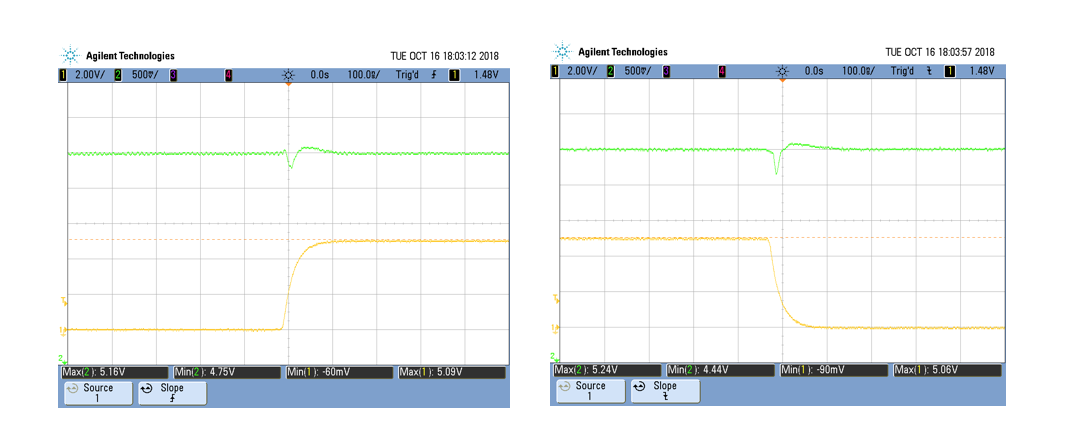
\includegraphics[scale=0.7]{../Exercise4/scap}
\caption{\color{cyan}Alimentation Voltage of the IC, with a ripple-response to an input signal's edge.}
\label{scap}
\end{figure}

It is seen in the osciloscope from Figure \ref{scap} that the alimentation voltage of the circuit in Figure \ref{comps} has a ripple when there is an edge of the square input signal. This is due to the big ammount of current that the integrated circuit of NOR gates demands from the voltage source when the input signal rises from 0V to 5V or when it falls from 5V to 0V. 
In order to reduce this "ripple-shape" response of the circuits to such edges, a capacitor has to be added between the +Vcc and the GND terminals of the integrated circuit. The goal is to add a capacitor in a way that the less inductance is added to the circuit. This capacitor has to be the nearest possible to such terminals, to avoid adding long wires that add inductance. Moreover,  the best capacitors' technology for this case is the multilayer capacitor as it doesn't add as much inductance as other technologies of this component. As it is preffered to use a multilayer capacitor between 10nF and 100nF for this situation, we decided to use a 100nF capacitor for the ripple to decrease, as it can be seen in Figure \ref{ccap}. By adding the capacitor, again, no significant temperature changes are noticed while varying the input signal's frequency, although when the circuit's capacitance increases, the dynamic power varies too.

\begin{figure}[h!]
\centering
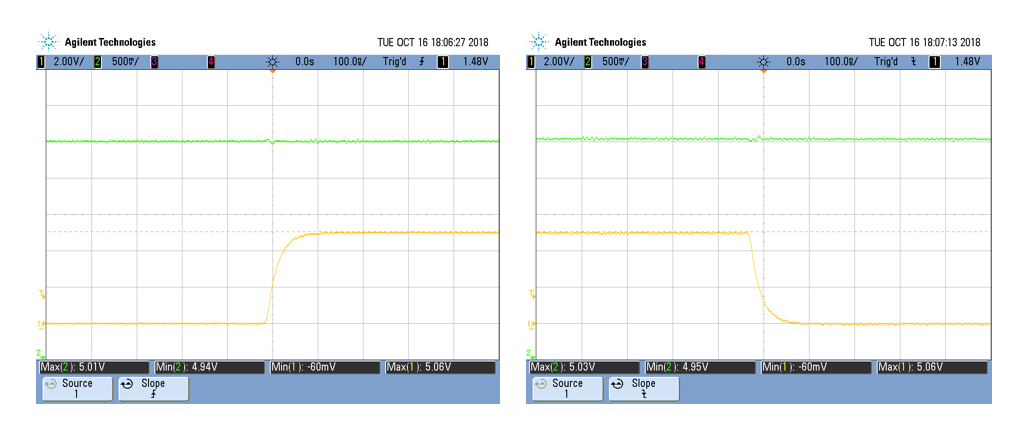
\includegraphics[scale=0.7]{../Exercise4/ccap}
\caption{\color{cyan}Alimentation Voltage of the IC with decoupling capacitor, with a smaller ripple-response to an input signal's edge.}
\label{ccap}
\end{figure}


%\end{document} 